% Options for packages loaded elsewhere
\PassOptionsToPackage{unicode}{hyperref}
\PassOptionsToPackage{hyphens}{url}
\PassOptionsToPackage{dvipsnames,svgnames,x11names}{xcolor}
%
\documentclass[
  letterpaper,
  DIV=11,
  numbers=noendperiod]{scrartcl}

\usepackage{amsmath,amssymb}
\usepackage{iftex}
\ifPDFTeX
  \usepackage[T1]{fontenc}
  \usepackage[utf8]{inputenc}
  \usepackage{textcomp} % provide euro and other symbols
\else % if luatex or xetex
  \usepackage{unicode-math}
  \defaultfontfeatures{Scale=MatchLowercase}
  \defaultfontfeatures[\rmfamily]{Ligatures=TeX,Scale=1}
\fi
\usepackage{lmodern}
\ifPDFTeX\else  
    % xetex/luatex font selection
\fi
% Use upquote if available, for straight quotes in verbatim environments
\IfFileExists{upquote.sty}{\usepackage{upquote}}{}
\IfFileExists{microtype.sty}{% use microtype if available
  \usepackage[]{microtype}
  \UseMicrotypeSet[protrusion]{basicmath} % disable protrusion for tt fonts
}{}
\makeatletter
\@ifundefined{KOMAClassName}{% if non-KOMA class
  \IfFileExists{parskip.sty}{%
    \usepackage{parskip}
  }{% else
    \setlength{\parindent}{0pt}
    \setlength{\parskip}{6pt plus 2pt minus 1pt}}
}{% if KOMA class
  \KOMAoptions{parskip=half}}
\makeatother
\usepackage{xcolor}
\setlength{\emergencystretch}{3em} % prevent overfull lines
\setcounter{secnumdepth}{-\maxdimen} % remove section numbering
% Make \paragraph and \subparagraph free-standing
\ifx\paragraph\undefined\else
  \let\oldparagraph\paragraph
  \renewcommand{\paragraph}[1]{\oldparagraph{#1}\mbox{}}
\fi
\ifx\subparagraph\undefined\else
  \let\oldsubparagraph\subparagraph
  \renewcommand{\subparagraph}[1]{\oldsubparagraph{#1}\mbox{}}
\fi


\providecommand{\tightlist}{%
  \setlength{\itemsep}{0pt}\setlength{\parskip}{0pt}}\usepackage{longtable,booktabs,array}
\usepackage{calc} % for calculating minipage widths
% Correct order of tables after \paragraph or \subparagraph
\usepackage{etoolbox}
\makeatletter
\patchcmd\longtable{\par}{\if@noskipsec\mbox{}\fi\par}{}{}
\makeatother
% Allow footnotes in longtable head/foot
\IfFileExists{footnotehyper.sty}{\usepackage{footnotehyper}}{\usepackage{footnote}}
\makesavenoteenv{longtable}
\usepackage{graphicx}
\makeatletter
\def\maxwidth{\ifdim\Gin@nat@width>\linewidth\linewidth\else\Gin@nat@width\fi}
\def\maxheight{\ifdim\Gin@nat@height>\textheight\textheight\else\Gin@nat@height\fi}
\makeatother
% Scale images if necessary, so that they will not overflow the page
% margins by default, and it is still possible to overwrite the defaults
% using explicit options in \includegraphics[width, height, ...]{}
\setkeys{Gin}{width=\maxwidth,height=\maxheight,keepaspectratio}
% Set default figure placement to htbp
\makeatletter
\def\fps@figure{htbp}
\makeatother

\KOMAoption{captions}{tableheading}
\makeatletter
\@ifpackageloaded{caption}{}{\usepackage{caption}}
\AtBeginDocument{%
\ifdefined\contentsname
  \renewcommand*\contentsname{Table of contents}
\else
  \newcommand\contentsname{Table of contents}
\fi
\ifdefined\listfigurename
  \renewcommand*\listfigurename{List of Figures}
\else
  \newcommand\listfigurename{List of Figures}
\fi
\ifdefined\listtablename
  \renewcommand*\listtablename{List of Tables}
\else
  \newcommand\listtablename{List of Tables}
\fi
\ifdefined\figurename
  \renewcommand*\figurename{Figure}
\else
  \newcommand\figurename{Figure}
\fi
\ifdefined\tablename
  \renewcommand*\tablename{Table}
\else
  \newcommand\tablename{Table}
\fi
}
\@ifpackageloaded{float}{}{\usepackage{float}}
\floatstyle{ruled}
\@ifundefined{c@chapter}{\newfloat{codelisting}{h}{lop}}{\newfloat{codelisting}{h}{lop}[chapter]}
\floatname{codelisting}{Listing}
\newcommand*\listoflistings{\listof{codelisting}{List of Listings}}
\makeatother
\makeatletter
\makeatother
\makeatletter
\@ifpackageloaded{caption}{}{\usepackage{caption}}
\@ifpackageloaded{subcaption}{}{\usepackage{subcaption}}
\makeatother
\ifLuaTeX
  \usepackage{selnolig}  % disable illegal ligatures
\fi
\usepackage{bookmark}

\IfFileExists{xurl.sty}{\usepackage{xurl}}{} % add URL line breaks if available
\urlstyle{same} % disable monospaced font for URLs
\hypersetup{
  colorlinks=true,
  linkcolor={blue},
  filecolor={Maroon},
  citecolor={Blue},
  urlcolor={Blue},
  pdfcreator={LaTeX via pandoc}}

\author{}
\date{2024-03-03}

\begin{document}

\subsection{5. Waagerechte und senkrechte
Asymptoten}\label{waagerechte-und-senkrechte-asymptoten}

\textbf{Bisher:} Wir haben hauptsächliche Ganzrationele Funktinen
betrachtet.\\
Es gibt aber auch Funktionen, mit ganzrationaler Funktion im Nenner,
z.B.: \[
f(x)=\frac{2x^2+1}{3x^3-x+1}
 \]

Dies Funktionen heißen \textbf{gebrochenrationale Funktionen}

\subparagraph{Definition:}\label{definition}

Funktionen der Art \(f(x)=\frac{g(x)}{h(x)}\), bei denen \(g\) und \(g\)
ganzrationele Funktionen sind und \(h\) einen Grad größer gleich 1 hat,
heißen \textbf{gebrochenrationale Funktionen}.

\subparagraph{Beispiele:}\label{beispiele}

\subparagraph{Beobachtung:}\label{beobachtung}

Ganzrationale Funktionen haben Definitionslücken, da nicht durch 0
geteilt werden darf.

Die Untersuchung und Angabe der Defintionsmenge ist folgliche
obligatorisch. Dafür reicht es aus den Nenner zu betrachten.

Wie verläuft der Graph bei sochen Definitionslücken?

\paragraph{Beispiel:}\label{beispiel}

\[
f(x)=\frac{2x^2+1}{3x^3-x+1}, \quad D=\mathbb{R} \setminus \{ -1\} 
 \]

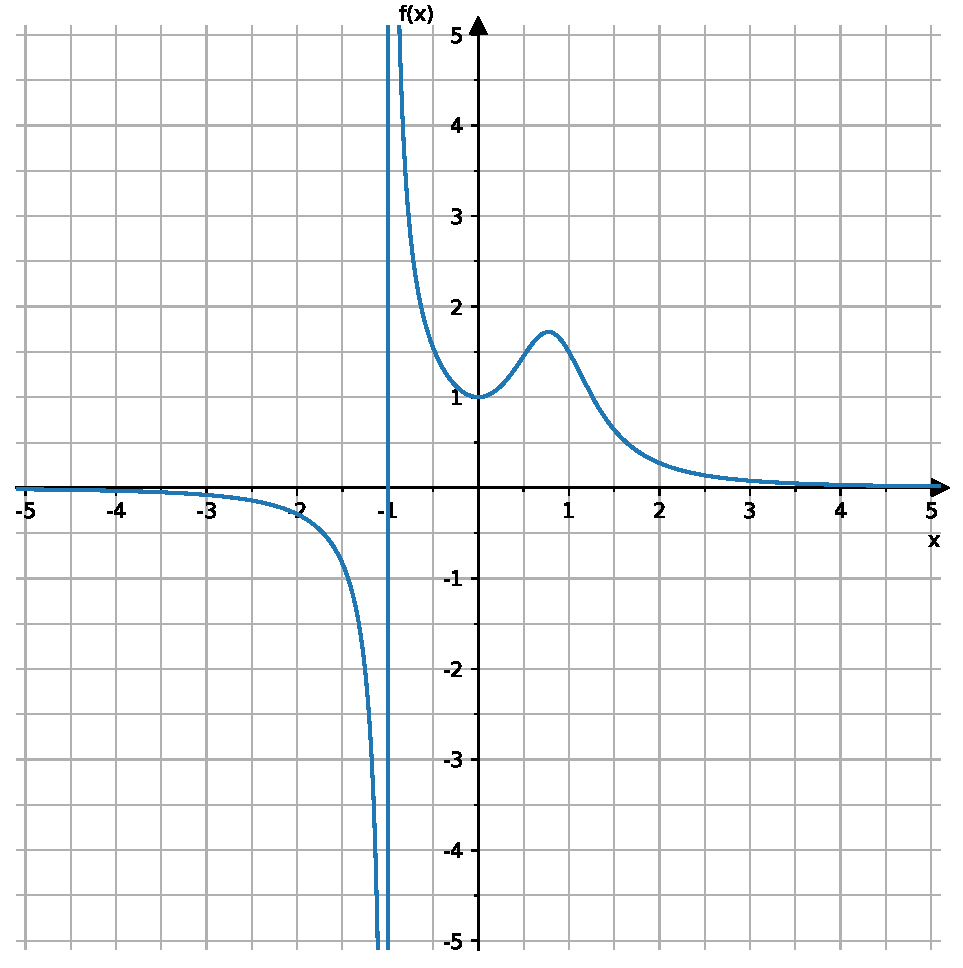
\includegraphics{5_Asymptoten_files/figure-pdf/cell-2-output-1.pdf}

\subparagraph{Beobachtung}\label{beobachtung-1}

Die Graphen von gebrochenrationalen Funktionen besitzen an den
Defintionslücken senkrechte Asymptoten.

\subparagraph{Untersuchung des Verhaltens an den
Definitionslücken}\label{untersuchung-des-verhaltens-an-den-definitionsluxfccken}

Idee: Man nähert sich in einer Umgebung der Defintionslücke von beiden
Seiten an und betrachtet die Veränderung der Funktionswerte.

\subparagraph{Beispiel:}\label{beispiel-1}

\[
\begin{aligned}
f(x)&=\frac{2x^2+1}{3x^3-x+1}, \quad D=\mathbb{R} \setminus \{ -1\} \\
\lim_{x \searrow -1} f(x) &= ?\\
\lim_{x \nearrow -1} f(x) &= ?\\
\end{aligned}\]

\(x \searrow -1\):

\begin{longtable}[]{@{}cc@{}}
\toprule\noalign{}
\(x\) & \(f(x)\) \\
\midrule\noalign{}
\endhead
\bottomrule\noalign{}
\endlastfoot
\(0\) & ? \\
\(-0,5\) & ? \\
\(-0,9\) & ? \\
\(-0,99\) & ? \\
\end{longtable}

\(x \nearrow -1\):

\begin{longtable}[]{@{}cc@{}}
\toprule\noalign{}
\(x\) & \(f(x)\) \\
\midrule\noalign{}
\endhead
\bottomrule\noalign{}
\endlastfoot
\(0\) & ? \\
\(-0,5\) & ? \\
\(-0,9\) & ? \\
\(-0,99\) & ? \\
\end{longtable}

\subparagraph{Satz:}\label{satz}

Gegeben: - ganzrationale Funktion \(f=\frac{g(x)}{h(x)}\) - \(g\) und
\(h\) differenzierbare Funktionen

Es gilt:

Wenn \(g(x_0)\neq 0\) und h(x\_0)=0\$ gilt, dann\\
- ist \(x_0\) eine \textbf{Polstelle} von \(f\) - Die Gerade mit der
Gleichung \(x=x_0\) ist eine senkrechte Asymptote von \(f\).

\subparagraph{Bemerkung:}\label{bemerkung}

\begin{itemize}
\tightlist
\item
  Der Pol ist die Stelle auf der x-Achse, durch welche die senkrechte
  Asmptote verläuft.
\item
  Man bezeichnet die Polstelle mit Vorzeichenwechsel, wenn einer der
  beiden ``Äste'' an der Senkrechten Asymptote gegen \(+ \infty\) und
  der andere gegen \(-\infty\) läuft.
\end{itemize}

So \(x\seqarrow -1\)

\begin{longtable}[]{@{}cc@{}}
\toprule\noalign{}
\(x\) & \(f(x)\) \\
\midrule\noalign{}
\endhead
\bottomrule\noalign{}
\endlastfoot
\(0\) & \\
\(-0,5\) & \\
\(-0,9\) & \\
\(-0,99\) & \\
\end{longtable}

\subparagraph{Forscheraufgabe}\label{forscheraufgabe}

Wenn die Voraussetzungen \(g(x_0)=0\) und gleichzeitig \(h(x_0)=0\)
erfüllt sind, lässt sich der Satz nicht anwenden!\\
Welche Aussgaben kann man dann machen? \(\Rightarrow\) Buch Seite 155
Nr. 13

\subparagraph{Beispiel:}\label{beispiel-2}

\[
f(x)=\frac{2x^2+1}{3x^3-x+1}, \quad D=\mathbb{R} \setminus \{ -1\} 
 \]

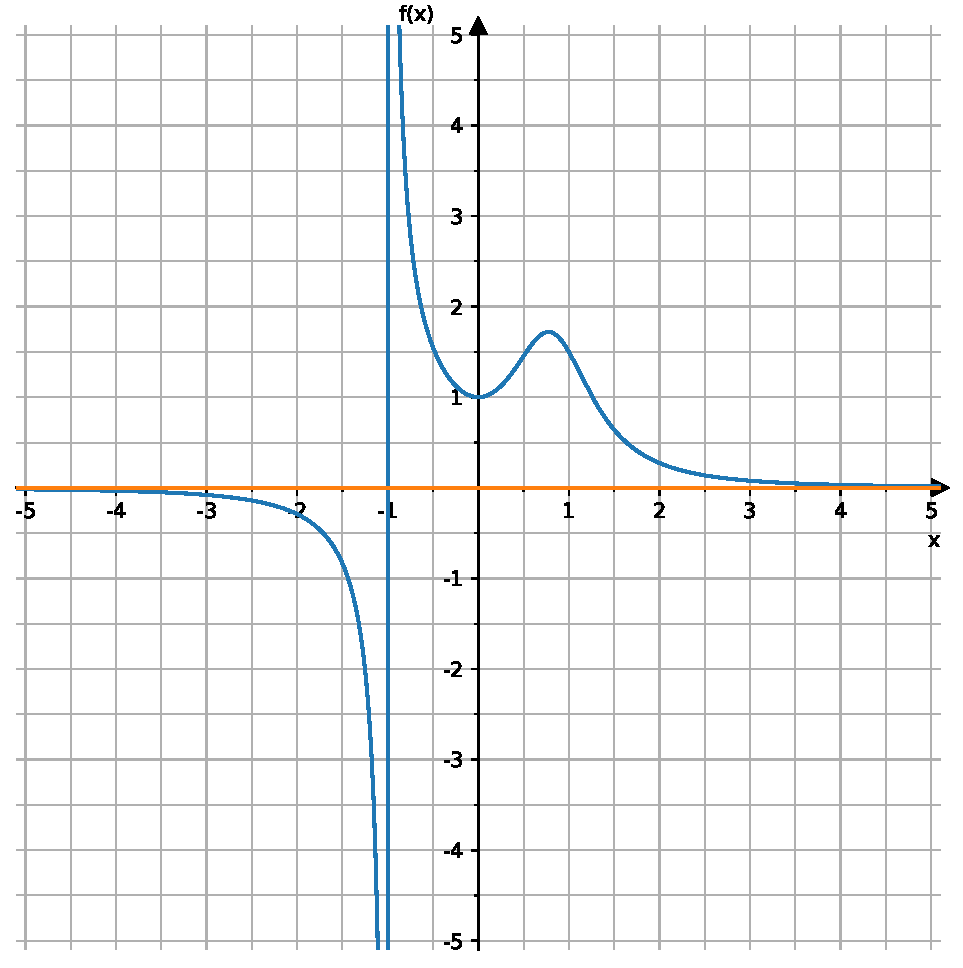
\includegraphics{5_Asymptoten_files/figure-pdf/cell-3-output-1.pdf}

\subparagraph{Beobachtung}\label{beobachtung-2}

\begin{itemize}
\tightlist
\item
  Es gibt auch waagerechte Asymptoten.
\item
  Waagerechte Asymptoten lassen sich mit Hilfe der Grenzwertbetrachtung
  suchen.
\end{itemize}

\subparagraph{Grenzwertbetrachtung}\label{grenzwertbetrachtung}

\[
 \begin{aligned}
f(x)&=\frac{2x^2+1}{3x^3-x+1}\\
& \lim_{x \to \infty}\frac{x^3\cdot \left( \frac{2}{x}+ \frac{1}{x^3} \right) }{x^3\cdot \left(3-\frac{1}{x^2}+\frac{1}{x^3}\right)}\\
&= \lim_{x \to \infty}\frac{\left( \frac{2}{x}+ \frac{1}{x^3} \right) }{\left(3-\frac{1}{x^2}+\frac{1}{x^3}\right)}\\
&=\frac{0}{3}\\
&= 0
\end{aligned}
 \]

\[
 \begin{aligned}
f(x)&=\frac{2x^2+1}{3x^3-x+1}\\
&\lim_{x \to -\infty}\frac{x^3\cdot \left( \frac{2}{x}+ \frac{1}{x^3} \right) }{x^3\cdot \left(3-\frac{1}{x^2}+\frac{1}{x^3}\right)}\\
&= \lim_{x \to -\infty}\frac{\left( \frac{2}{x}+ \frac{1}{x^3} \right) }{\left(3-\frac{1}{x^2}+\frac{1}{x^3}\right)}\\
&=\frac{0}{3}\\
&= 0
\end{aligned}
 \]

\subparagraph{Beobachtung}\label{beobachtung-3}

\begin{itemize}
\tightlist
\item
  Der Graph nähert sich für \(x \rightarrow \pm \infty\) der Geraden mit
  der Gleichung \(y=0\) an.
\item
  Diese Gerade heißt waagerechte Asymptote
\end{itemize}

\subparagraph{Satz:}\label{satz-1}

Gegeben: - ganzrationale Funktion \(f=\frac{g(x)}{h(x)}\) - der Grad des
Zählers \(g\) sei \(a\) - der Grad des Nenners \(h\) sei \(b\).

Es gilt:

\begin{itemize}
\tightlist
\item
  \(a < b\): waagerechte Asymptote mit \(y=0\).
\item
  \(a = b\): waagerechte Asymptote mit \(y=\frac{a}{b}\)
\item
  \(a > b\): keine waagerechte Asymptote.
\end{itemize}



\end{document}
